\section{Output of Graphviz's layout on a hotword detection model used at Snips.}
\label{appendix-graphviz}
\begin{center}
\vspace{-0.5em}
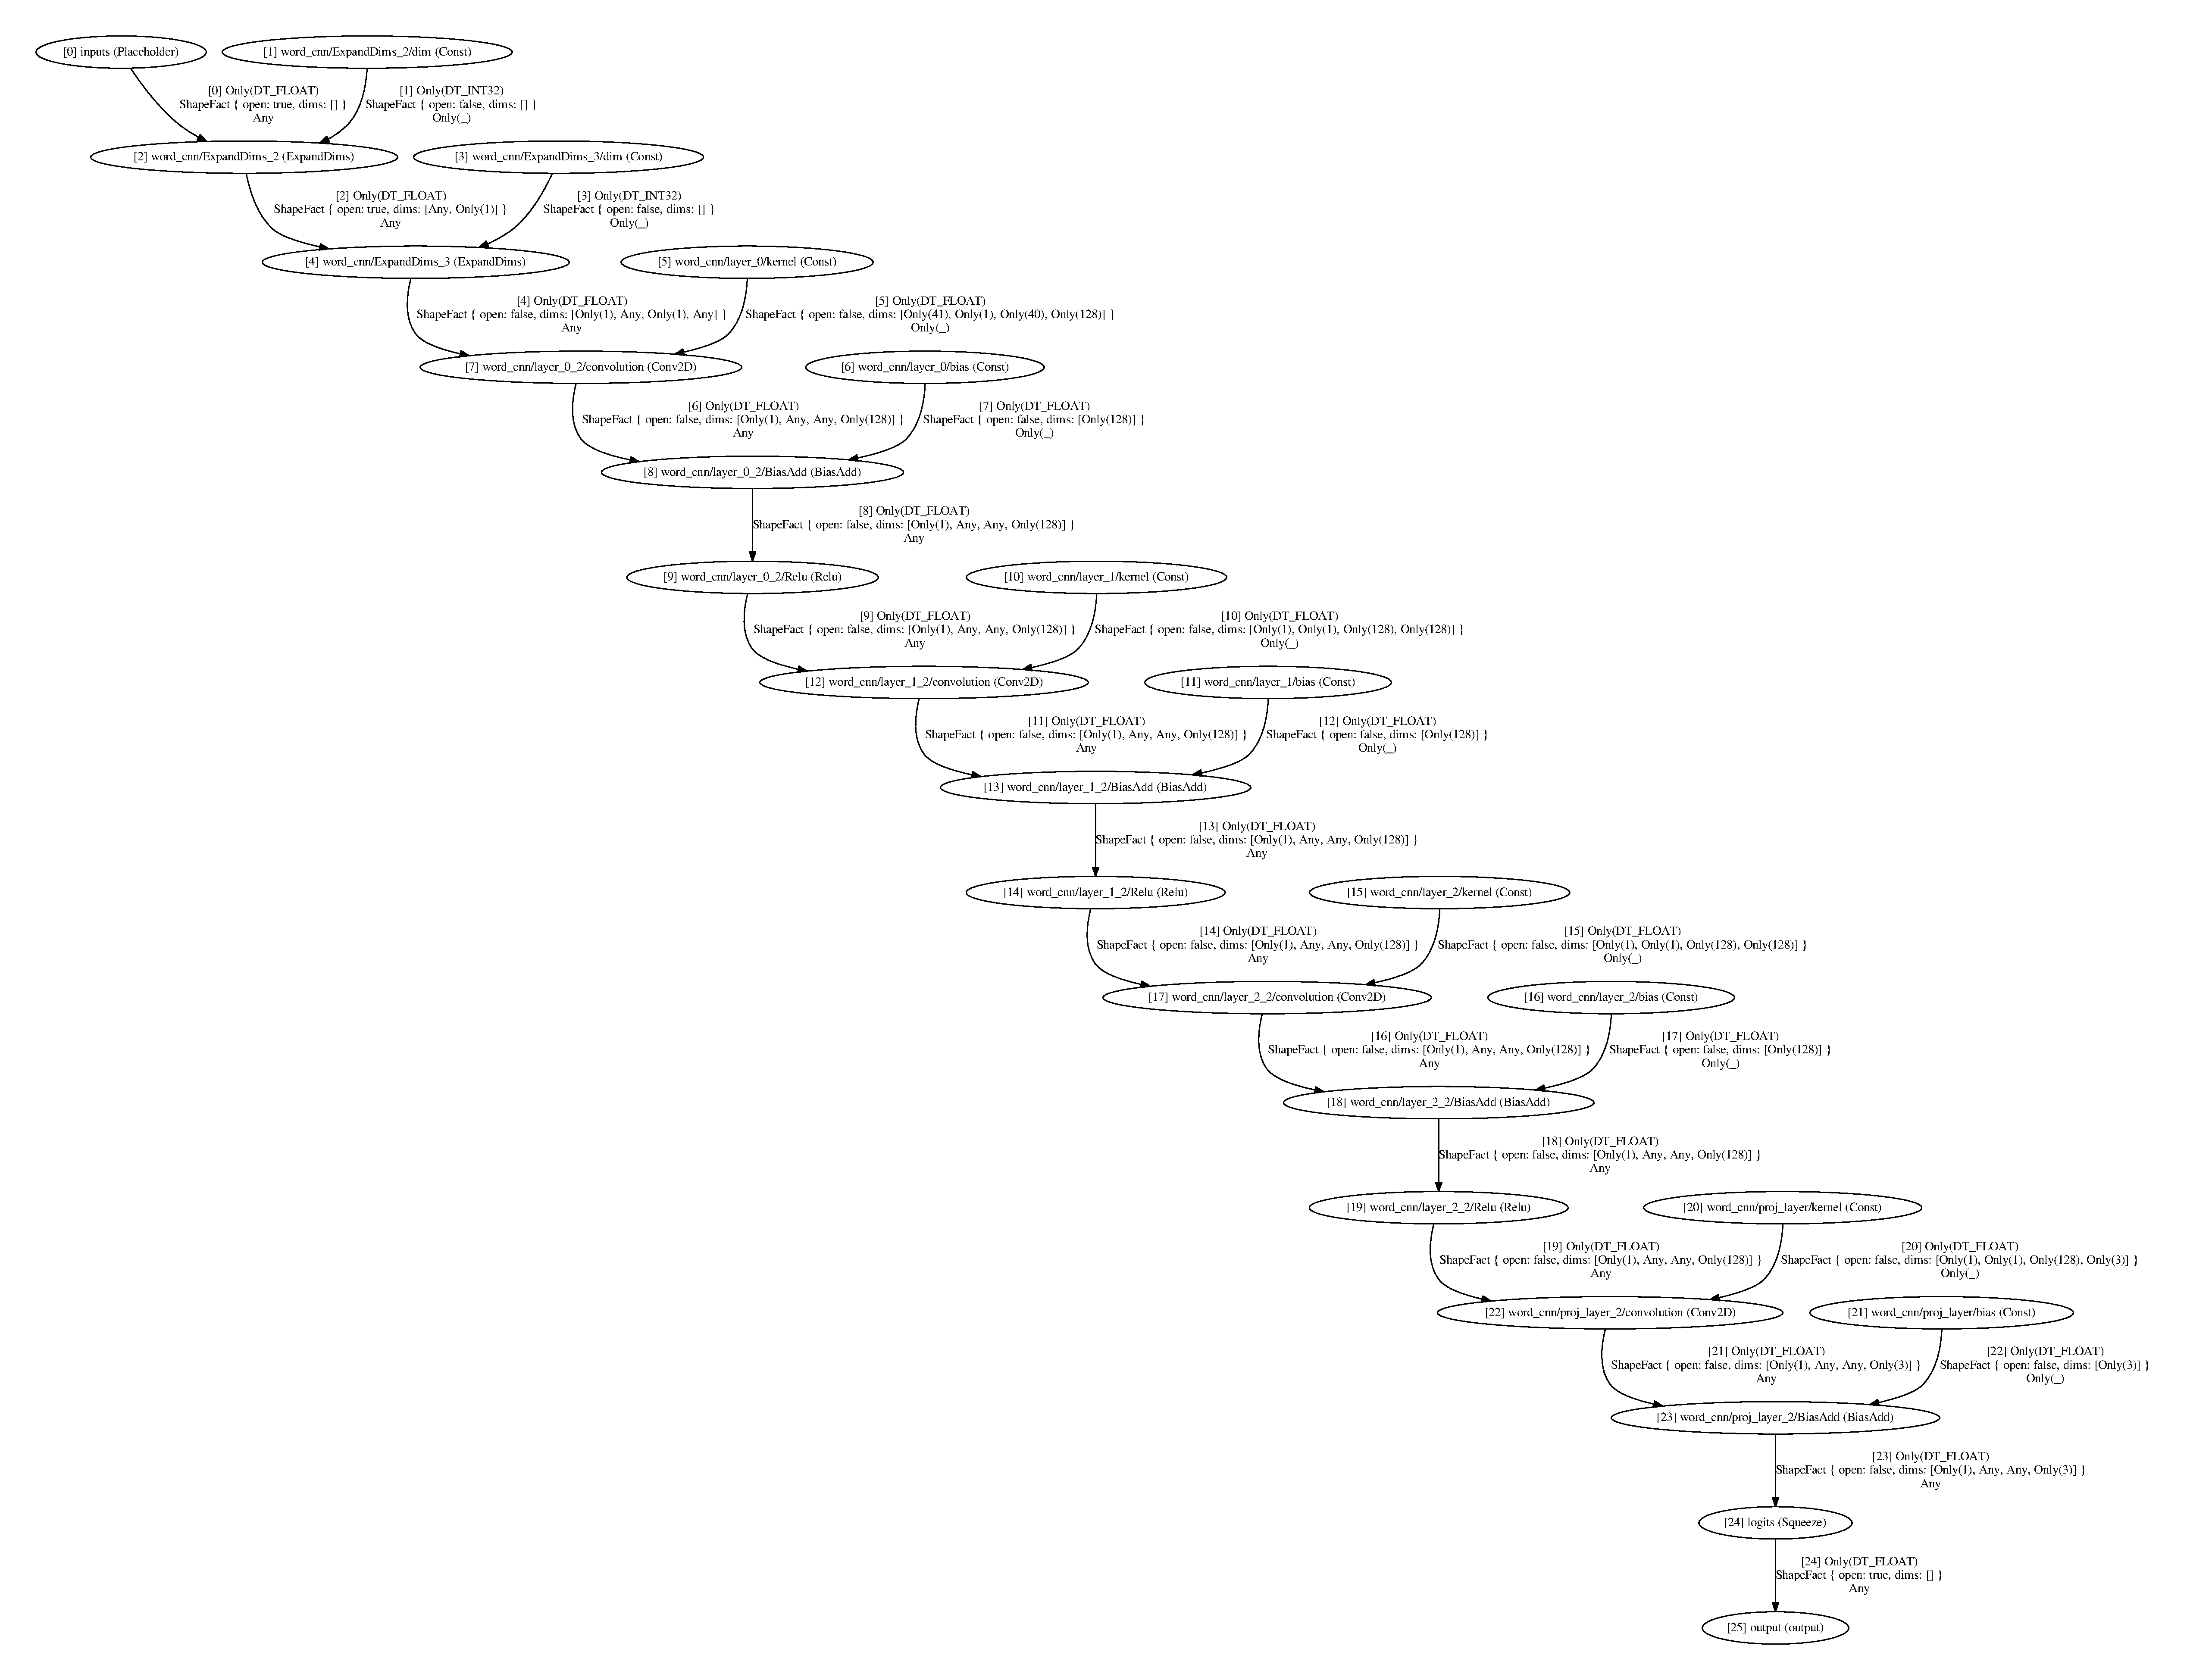
\includegraphics[width=\textwidth]{hotword-classic-graphviz.pdf}
\vspace{-1em}
\end{center}

\newpage
\section{Type definitions and unification functions for the analyser facts.}
\label{appendix-analyser-types}
\setminted{fontsize=\footnotesize,baselinestretch=1}
\inputminted{rust}{analyser-types.rs}

\bigskip
\appendixref{Edited for clarity, see the full version at \url{https://github.com/kali/tensorflow-deploy-rust/blob/master/src/analyser/types.rs}.}

\newpage
\section{Rust implementation of the propagation algorithm.}
\label{appendix-analyser-algorithm}
\setminted{fontsize=\footnotesize,baselinestretch=1}
\inputminted{rust}{analyser-algorithm.rs}

\newpage
\section{Previous implementation of ${enrich^\rightarrow}_\texttt{Pad}$.}
\label{appendix-analyser-pad-code}
\setminted{fontsize=\footnotesize,baselinestretch=1}
\begin{minted}{rust}
/// Deduces properties about the output tensors from the input tensors.
fn enrich_forward(&self, mut inputs: Vec<&TensorFact>) -> Result<Option<Vec<TensorFact>>> {
    use analyser::*;

    if inputs.len() != 2 {
        bail!("Pad operation needs exactly two inputs.");
    }

    // If we know everything about all the input ports.
    if let Some(output) = infer_forward_concrete(self, &inputs)? {
        return Ok(Some(output));
    }

    let (input_fact, paddings_fact) = args_2!(inputs);

    // If we know the type of the input, we can deduce the type of the output.
    let mut output_fact = TensorFact {
        datatype: input_fact.datatype,
        ..TensorFact::default()
    };

    // If we know the shape of the input and the value of paddings, we can
    // deduce the shape of the output.
    if let (Some(mut shape), Some(pad)) =
           (input_fact.shape.concretize(), paddings_fact.value.concretize()) {
        let pad = i32::tensor_to_view(pad)?;
        shape.iter_mut()
            .zip(pad.outer_iter())
            .for_each(|(s, p)| *s += p[0] as usize + p[1] as usize);
        
        output_fact.shape = shape.into();
    }

    Ok(Some(vec!(output_fact)))
}
\end{minted}

\bigskip
\appendixref{Edited for clarity, see the full version at \url{https://github.com/kali/tensorflow-deploy-rust/blob/5e73c94f60aef4ccf1b3c63af180a13cc4567a3b/src/ops/array/pad.rs}.}

\newpage
\section{Rust implementation of the declarative constraint solver.}
\label{appendix-analyser-solver-impl}
\setminted{fontsize=\footnotesize,baselinestretch=1}
\inputminted{rust}{analyser-solver.rs}

\newpage
\section{Solver rules for \texttt{Pad} \textit{(Rust code)}.}
\label{appendix-analyser-pad-rules}
\setminted{fontsize=\footnotesize,baselinestretch=1}

\begin{minted}{rust}
impl<T: Datum> InferenceRulesOp for Pad<T> {
    fn rules(&self, inputs, outputs) {
        let input = &inputs[0];
        let paddings = &inputs[1];
        let output = &outputs[0];

        solver
            .equals(&inputs.len, 2)
            .equals(&outputs.len, 1)
            .equals(&output.datatype, &input.datatype)
            .equals(&paddings.datatype, DataType::DT_INT32)
            .equals(&input.rank, &output.rank)
            .equals(&paddings.rank, 2)
            .equals(&paddings.shape[0], &input.rank)
            .equals(&paddings.shape[1], 2)
            .given(&input.rank, move |solver, rank: usize| {
                (0..rank).for_each(|i| {
                    solver.equals_zero(wrap!(
                        (-1, &output.shape[i]),
                        (1, &input.shape[i]),
                        (1, &paddings.value[i][0]),
                        (1, &paddings.value[i][1])
                    ));
                })
            })
        ;
    }
}
\end{minted}

\newpage
\section{Rust implementation of the constant folding algorithm.}
\label{appendix-analyser-constants}
\setminted{fontsize=\footnotesize,baselinestretch=1}
\inputminted{rust}{analyser-constants.rs}

\newpage
\section{Rust implementation of $step_\texttt{Conv2D}$.}
\label{appendix-streaming-conv2d}
\setminted{fontsize=\footnotesize,baselinestretch=1}

\inputminted{rust}{streaming-conv2d.rs}
\bigskip
\appendixref{Edited for clarity, see the full version at \url{https://github.com/kali/tensorflow-deploy-rust/blob/master/src/ops/nn/conv2d.rs}.}

\newpage
\section{Rust implementation of the streaming inference algorithm.}
\label{appendix-streaming-algorithm}
\setminted{fontsize=\footnotesize,baselinestretch=1}

\inputminted{rust}{streaming-algorithm.rs}
\bigskip
\appendixref{Edited for clarity, see the full version at \url{https://github.com/kali/tensorflow-deploy-rust/blob/master/src/lib.rs}.}
